%%%%%%%%%%%%%%%%%%%%%%%%
% MinGW
%%%%%%%%%%%%%%%%%%%%%%%%

\subsubsection{Purpose}
\noindent \ac{EMTG} depends on the \ac{SNOPT} \ac{NLP} solver package, which is written in Fortran, and MinGW provides a free Fortran compiler and runtime library for Windows. These instructions assume that MinGW is used to compile the \ac{SNOPT} library used by \ac{EMTG}. \\ \ac{EMTG} is known to work with \hl{MinGW 7.2.0}.

\subsubsection{Download Location}
\noindent The main page for the software distributions is in the following website: \\
\url{https://sourceforge.net/projects/mingw-w64/files/}

\noindent The software package needed for the EMTG version indicated in this guide can be obtained from the following location:
\emph{(In the event the url is no longer active, navigate to the aforementioned software website to find the specific version)} \\ \url{https://sourceforge.net/projects/mingw-w64/files/Toolchains%20targetting%20Win64/Personal%20Builds/mingw-builds/7.2.0/threads-posix/seh/x86_64-7.2.0-release-posix-seh-rt_v5-rev1.7z/download}

\subsubsection{Dependency Installation Instructions}
\label{sec:mingw_installation_instructions}
\begin{enumerate}
	\item Unzip the file downloaded into a desired folder location for later use in an upcoming step. 
	\begin{enumerate}
		\item Install 7zip if that is not already installed on your machine to extract the *.7z file. 
	\end{enumerate}	
	\item Edit the user’s Path environment variable to include the bin directory of MinGW so that the EMTG executable can find the Fortran runtime library during execution.
	\begin{enumerate}
		\item Press the Windows button.
		\item Type “Edit environment variables for your account”. %\\ \emph{(Autocomplete may take over at some point.)} 
		\begin{figure}[H]
			\centering
			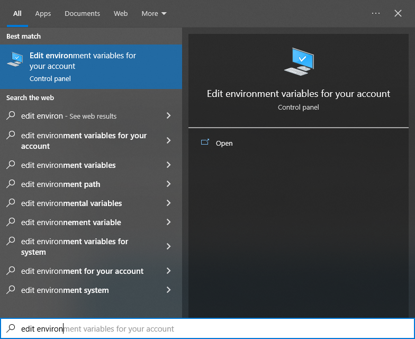
\includegraphics[width=0.7\linewidth]{../../../shared_latex_inputs/images/windows_env-variables_launch.png}
			\caption{Launching Windows Environment Variables Menu}
		\end{figure}
		\item In the upper block of the new window, labeled “User variables for [User]”, click on “Path”, then click on the “Edit...” button. 
		\begin{figure}[H]
			\centering
			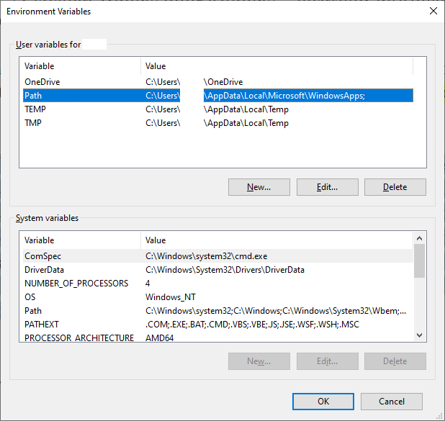
\includegraphics[width=0.7\linewidth]{../../../shared_latex_inputs/images/windows_env-variables_menu.png}
			\caption{Windows Environment Variables Menu}
		\end{figure}
		\item In the popup window, click “New”. In the new line, type the full path to the MinGW bin directory. 
		\begin{figure}[H]
			\centering
			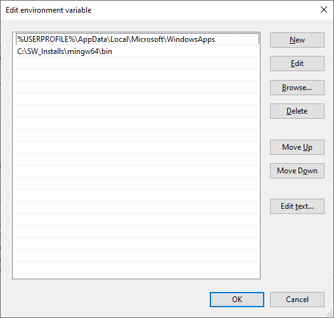
\includegraphics[width=0.7\linewidth]{../../../shared_latex_inputs/images/windows_env-variables_path.png}
			\caption{Windows Edit Environment Variable Menu}
		\end{figure}
		An example of the MinGW path would be 
		\begin{verbatim}
			C:\SW_Installs\mingw64\bin
		\end{verbatim}
		\item Click the OK button in both dialog windows to save the edit to the Path.
	\end{enumerate}		
\end{enumerate}

